\chapter{Application dédiée}
\section{Introduction}
Nous allons maintenant présenter une application qui va utiliser le système présenté précédemment. Une interface homme-machine connecté avec un agent central (centre de ventes) ainsi que plusieurs agents annexes (vendeurs). dans notre cas tous les agents sont dans le même serveur et connectés à une même base de données.
Le centre de vente est spécialisé dans la vente des vêtements. Chaque vendeur s'occupe d'une catégorie de vêtement: pantalon, t-shirt, chaussures etc.
\section{Interface homme-machine}
Nous passons à présent à l’interface graphique du centre de ventes. Celle si a deux composantes principales:
\begin{itemize}
	\item Fenêtre pour la requête.
	\item Fenêtre pour le résultat de la requête.
\end{itemize}
Ainsi qu’une partie pour simuler l’ajout d’agents.
\begin{figure}[H]
	\centering
	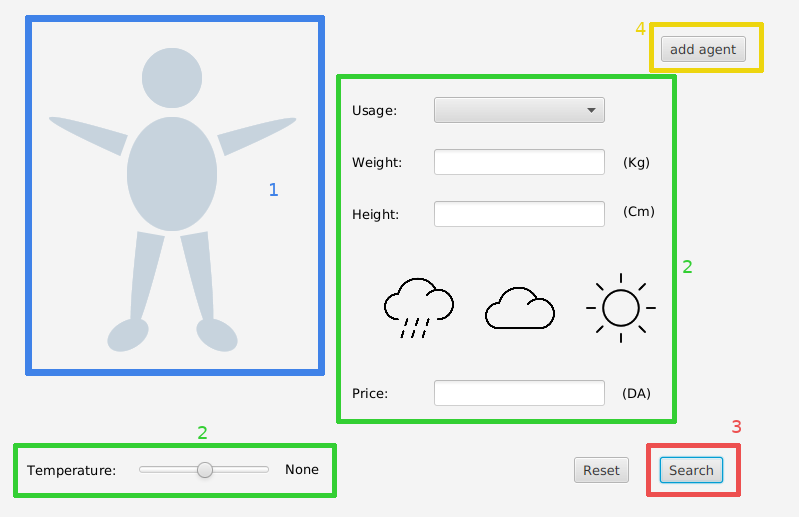
\includegraphics[scale=0.4]{imgs/agentUI1.png}
	\caption{Fenêtre dédiée à la formulation de requêtes}
	\label{fig:queryWin}
\end{figure}
L’interface si dessus contient 4 parties:
\begin{enumerate}
	\item Sélectionner la partie du corps que doit couvrir le produit dont on est intéressé.
	\item Les différents attributs qu’on peut spécifier afin de préciser les détails concernant le produit à acheter:
	\begin{itemize}
		\item Utilisation du produit.
		\item Poids et taille de l’intéressé.
		\item La saison du produit.
		\item Prix du produit.
	\end{itemize}
	\item Bouton de recherche: après avoir fini de formuler la requête, ce bouton permet de l’envoyer aux agents annexes.
	\item Bouton ajouter agent: permet de simuler le fait qu’un ajout rejoigne le système, la figure si dessous montre qu’on peut donner à cet agent une catégorie de vêtements selon leur position dans le corps.
\end{enumerate}
\begin{figure}[H]
	\centering
	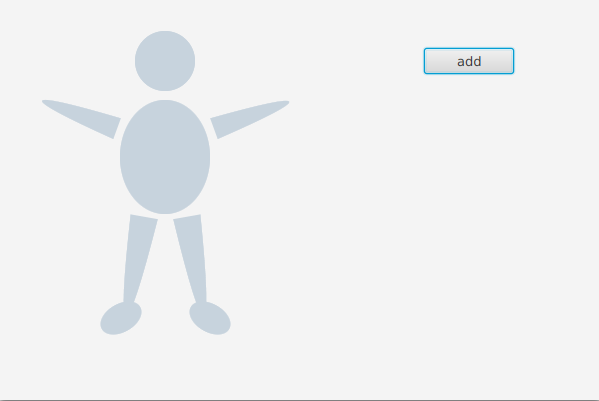
\includegraphics[scale=0.4]{imgs/agentUI3.png}
	\caption{Fenêtre dédiée à l'ajout d'agent au système}
	\label{fig:addAgent}
\end{figure}
\newpage
Et enfin la fenêtre qui permet d’afficher le résultat de la requête:
\begin{figure}[H]
	\centering
	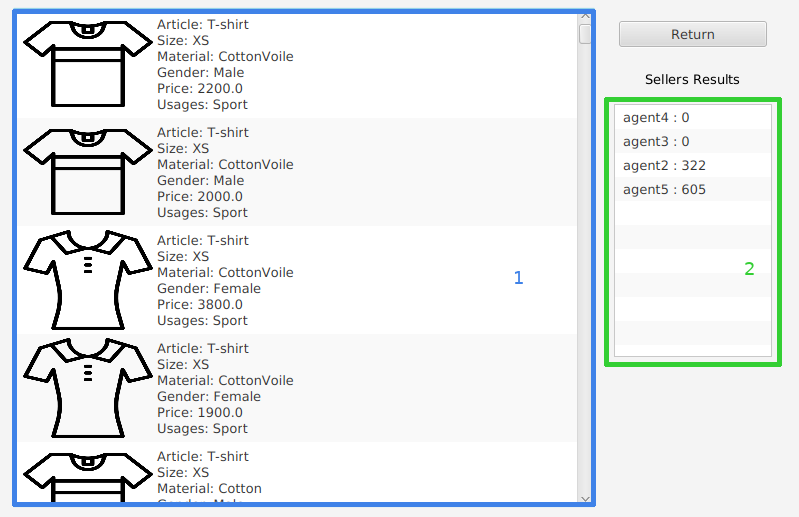
\includegraphics[scale=0.4]{imgs/agentUI2.png}
	\caption{Fenêtre dédiée aux résultats des requêtes}
	\label{fig:queryResult}
\end{figure}
On peut séparer cette fenêtre en deux parties:
\begin{enumerate}
	\item Partie pour l’affichage des produits résultats.
	\item Partie pour l’affichage des agents contactés ainsi que le nombre de produits communiqués par ces agents.
\end{enumerate}



